I eksempel \ref{ex:car2} med trafikken i et vejkryds blev tiden mellem to bilers ankomst modelleret med en eksponentielfordelt tilfældig variabel $T$ med parametren $\lambda = 1/60^2$ s$^{-1}$. Lad nu $T_1, T_2, \dots$ være forskellige tilfældige variable der modellerer tiden mellem hver bil over en tidsperiode, eksempelvis en dag, således $T_i \sim \exp(\lambda)$ for $i = 0,1,\dots$. Ankomsttidspunkter over en hel dag er da en såkaldt \emph{punkt process}, hvor hvert punkt markerer ankomstentidspunktet for en bil (se figur \ref{fig:process1}).
\begin{figure}[H]
\centering
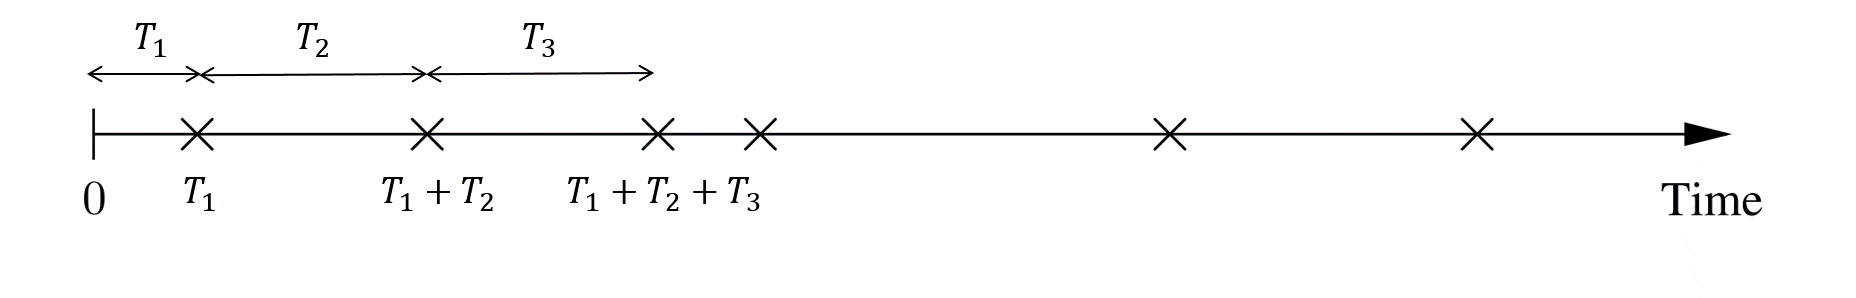
\includegraphics[width = \textwidth]{process1.png}
\caption{Punktprocess hvor $\times$ markerer hændelser i tid, eksempelvis ankomsttidspunkter af biler i et trafikkryds.} \label{fig:process1}
\end{figure}
I det specielle tilfælde hvor $T_1, T_2, \dots$ er eksponentielfordelte med parameter $\lambda$, da er punkt processen den såkaldte \emph{Poisson process}. Poisson processen er nytting til at modellere processer hvor ankomster i tid sker tilfældigt og uafhængigt i tid. Andre eksempler kunne være ankomst af opgaver til en computerserver, kø på apoteket, tidspunkter for jordskælv, ulykker på motervej og henfald af radioaktive partikler.
\\ \\  
Følgende resultat om Possion processer er nyttigt og giver den sammenhæng vi tidligere så mellem Possion og eksponentiel fordelingen. Lad $X(t)$ være en tilfældig variabel der tæller antallet af punkter fra $0$ til $t$ i en Poisson process med parameter $\lambda$. Det viser sig da at $X(t)$ følger en Possion fordeling med parameteren $t \lambda $. Den forventede værdi af $X(t)$ er dermed $E[X(t)] = t \lambda$. $\lambda$ kan således tolkes som antal forventede hændelser per tidsenhed og kaldes af denne grund \emph{raten}. 
\begin{example}
I en lufthavn ankommer hvert døgn gennemsnitligt $400$ fly. Flyene ankommer tilfældigt i løbet af døgnet og er ikke koordineret flyene imellem. Ud fra disse oplysninger kan vi antage en Poisson process for ankomsttidspunkter. Hvis $X(t)$ er antallet af fly i løbet af t timer vil denne følge en Poisson fordeling hvor:
\begin{align*}
E[X(24)] = 24\lambda = 400 \Rightarrow \lambda = 400/24 \approx 16.7,
\end{align*}
således $X(t) \sim \text{Poi}(16.7\cdot t)$ og $T_i \sim \exp(16.7)$. Da tiden mellem to flyvere $T_i$ er eksponentielfordelt med parameter $16.7$ da vil den forventede tid være $E[T_i] = 1/16.7 = 0.06$ timer $= 3.6$ minutter med en standardafvigelse også på $3.6$ minutter. 
\end{example}
Et andet nyttigt resultat kan bruges til nemt at simulere en Poisson process. Vi har givet en Poisson process med rate $\lambda$. Givet at der er $N$ antal punkter i tidsperioden $[0,t]$ vil fordelingen for tidspunkterne være uafhængigt uniformt fordelte tilfældige variable i intervallet $[0,t]$. Kender vi $N$ kan man altså blot simulere $N$ punkter uniformt fordelt i intervallet $[0,t]$ for at simulere en Poisson process. De to resultater om Poisson processen kan således bruges til at simulere dem, hvilket er opsummeret i algoritme \ref{alg:poisprocss}. Se \cite[240-247]{olofsson2012} for mere om Poisson processer. 
\begin{algorithm}
\begin{algorithmic}
\STATE Simuler $N \sim \text{Poi}(t\lambda)$ 
\FOR{$i = 0$ til $N-1$}
\STATE Simuler $Y_i \sim \text{unif}(0,t)$ \COMMENT{$Y_i$ er tidspunktet for en hændelse}
\ENDFOR 
\end{algorithmic}
\caption{Simulering af Poisson process med rate $\lambda$ mellem $0$ og $t$} \label{alg:poisprocss}
\end{algorithm}